\pdfoutput=1
\pdfcompresslevel=9
\pdfinfo
{
    /Author (Autor)
    /Title (Tytul)
    /Subject (Tematyka)
    /Keywords (Slowa kluczowe)
}
%\documentclass[a4paper,polish,onecolumn,oneside,floatssmall,11pt,titleauthor,wide,openright]{mwrep}
%\usepackage[scale={0.7,0.8},paper=a4paper,twoside]{geometry}
\documentclass[a4paper,onecolumn,oneside,11pt,wide,floatssmall]{mwrep}
% \usepackage{polish}
\usepackage{amsmath}
\usepackage{amsfonts}
\usepackage{amssymb}
\usepackage{amsthm}
\usepackage{bookman}

\usepackage{geometry}
\usepackage[utf8x]{inputenc}
\usepackage[T1]{fontenc}
% \usepackage{t1enc}
% \usepackage[pdftex, bookmarks]{hyperref}
\usepackage[pdftex, bookmarks=false]{hyperref}
\def\url#1{{ \tt #1}}

\usepackage{listings}

% marginesy
\textwidth\paperwidth
\advance\textwidth -55mm
\oddsidemargin-0.9in
\advance\oddsidemargin 33mm
\evensidemargin-0.9in
\advance\evensidemargin 33mm
\topmargin -1in
\advance\topmargin 25mm
\setlength\textheight{48\baselineskip}
\addtolength\textheight{\topskip}
\marginparwidth15mm

\clubpenalty=10000 % to kara za sierotki
\widowpenalty=10000 % nie pozostawia wdów
\brokenpenalty=10000 % nie dzieli wyrazów pomiędzy stronami
\sloppy

\tolerance4500
\pretolerance250
\hfuzz=1.5pt
\hbadness1450

% ŻYWA PAGINA
\renewcommand{\chaptermark}[1]{\markboth{\scshape\small\bfseries \
#1}{\small\bfseries \ #1}}
\renewcommand{\sectionmark}[1]{\markboth{\scshape\small\bfseries\thesection.\
#1}{\small\bfseries\thesection.\ #1}}
\newcommand{\headrulewidth}{0.5pt}
\newcommand{\footrulewidth}{0.pt}
\pagestyle{uheadings}

\usepackage[pdftex]{color,graphicx}
\usepackage[polish]{babel}

% \textheight232mm
% \setlength{\textwidth}{\textwidth}
% \setlength{\oddsidemargin}{\evensidemargin}
% \setlength{\evensidemargin}{0.3cm}
\usepackage[sort, compress]{cite}

%\usepackage{multibib}
%\newcites{bk,st,doc,web}{Książki i~artykuły,Standardy i~zalecenia,Dokumentacja produktów,Publikacje i~serwisy internetowe}

\theoremstyle{definition}
\newtheorem{defn}{Definicja}[section]
\newtheorem{conj}{Teza}[section]
\newtheorem{conjmain}{Teza}
\newtheorem{exmp}{Przykład}[section]

\theoremstyle{plain}% default
\newtheorem{thm}{Twierdzenie}[section]
\newtheorem{lem}[thm]{Lemat}
\newtheorem{prop}[thm]{Hipoteza}
\newtheorem*{cor}{Wniosek}

\theoremstyle{remark}
\newtheorem*{rem}{Uwaga}
\newtheorem*{note}{Uwaga}
\newtheorem{case}{Przypadek}

\definecolor{ListingBackground}{rgb}{0.95,0.95,0.95}

\begin{document}

% kody źródłowe wplatane w tekst
\lstdefinestyle{incode}
{
basicstyle={\footnotesize},
keywordstyle={\bf\footnotesize\color{blue}},
commentstyle={\em\footnotesize\color{magenta}},
numbers=left,
stepnumber=5,
firstnumber=1,
numberfirstline=true,
numberblanklines=true,
numberstyle={\sf\tiny},
numbersep=10pt,
tabsize=2,
xleftmargin=17pt,
framexleftmargin=3pt,
framexbottommargin=2pt,
framextopmargin=2pt,
framexrightmargin=0pt,
showstringspaces=true,
backgroundcolor={\color{ListingBackground}},
extendedchars=true,
% title=\lstname,
captionpos=b,
% abovecaptionskip=1pt,
% belowcaptionskip=1pt,
frame=tb,
framerule=0pt,
}

% kody źródłowe z podpisem
\lstdefinestyle{outcode}
{
basicstyle={\footnotesize},
keywordstyle={\bf\footnotesize\color{blue}},
commentstyle={\em\footnotesize\color{magenta}},
numbers=left,
stepnumber=5,
firstnumber=1,
numberfirstline=true,
numberblanklines=true,
numberstyle={\sf\tiny},
numbersep=10pt,
tabsize=2,
xleftmargin=17pt,
framexleftmargin=3pt,
framexbottommargin=2pt,
framextopmargin=2pt,
framexrightmargin=0pt,
showstringspaces=true,
backgroundcolor={\color{ListingBackground}},
extendedchars=true,
% title=\lstname,
captionpos=b,
% abovecaptionskip=1pt,
% belowcaptionskip=1pt,
frame=tb,
framerule=0.1pt,
}

\renewcommand*\lstlistingname{Wydruk}
\renewcommand*\lstlistlistingname{Spis wydruków}

\pagenumbering{roman}
\renewcommand{\baselinestretch}{1.0}
\raggedbottom
\pdfoutput=1
\pdfcompresslevel=9
\pdfinfo
{
    /Author (Autor)
    /Title (Tytul)
    /Subject (Tematyka)
    /Keywords (Slowa kluczowe)
}
%\documentclass[a4paper,polish,onecolumn,oneside,floatssmall,11pt,titleauthor,wide,openright]{mwrep}
%\usepackage[scale={0.7,0.8},paper=a4paper,twoside]{geometry}
\documentclass[a4paper,onecolumn,oneside,11pt,wide,floatssmall]{mwrep}
% \usepackage{polish}
\usepackage{amsmath}
\usepackage{amsfonts}
\usepackage{amssymb}
\usepackage{amsthm}
\usepackage{bookman}

\usepackage{geometry}
\usepackage[utf8x]{inputenc}
\usepackage[T1]{fontenc}
% \usepackage{t1enc}
% \usepackage[pdftex, bookmarks]{hyperref}
\usepackage[pdftex, bookmarks=false]{hyperref}
\def\url#1{{ \tt #1}}

\usepackage{listings}

% marginesy
\textwidth\paperwidth
\advance\textwidth -55mm
\oddsidemargin-0.9in
\advance\oddsidemargin 33mm
\evensidemargin-0.9in
\advance\evensidemargin 33mm
\topmargin -1in
\advance\topmargin 25mm
\setlength\textheight{48\baselineskip}
\addtolength\textheight{\topskip}
\marginparwidth15mm

\clubpenalty=10000 % to kara za sierotki
\widowpenalty=10000 % nie pozostawia wdów
\brokenpenalty=10000 % nie dzieli wyrazów pomiędzy stronami
\sloppy

\tolerance4500
\pretolerance250
\hfuzz=1.5pt
\hbadness1450

% ŻYWA PAGINA
\renewcommand{\chaptermark}[1]{\markboth{\scshape\small\bfseries \
#1}{\small\bfseries \ #1}}
\renewcommand{\sectionmark}[1]{\markboth{\scshape\small\bfseries\thesection.\
#1}{\small\bfseries\thesection.\ #1}}
\newcommand{\headrulewidth}{0.5pt}
\newcommand{\footrulewidth}{0.pt}
\pagestyle{uheadings}

\usepackage[pdftex]{color,graphicx}
\usepackage[polish]{babel}

% \textheight232mm
% \setlength{\textwidth}{\textwidth}
% \setlength{\oddsidemargin}{\evensidemargin}
% \setlength{\evensidemargin}{0.3cm}
\usepackage[sort, compress]{cite}

%\usepackage{multibib}
%\newcites{bk,st,doc,web}{Książki i~artykuły,Standardy i~zalecenia,Dokumentacja produktów,Publikacje i~serwisy internetowe}

\theoremstyle{definition}
\newtheorem{defn}{Definicja}[section]
\newtheorem{conj}{Teza}[section]
\newtheorem{conjmain}{Teza}
\newtheorem{exmp}{Przykład}[section]

\theoremstyle{plain}% default
\newtheorem{thm}{Twierdzenie}[section]
\newtheorem{lem}[thm]{Lemat}
\newtheorem{prop}[thm]{Hipoteza}
\newtheorem*{cor}{Wniosek}

\theoremstyle{remark}
\newtheorem*{rem}{Uwaga}
\newtheorem*{note}{Uwaga}
\newtheorem{case}{Przypadek}

\definecolor{ListingBackground}{rgb}{0.95,0.95,0.95}

\begin{document}

% kody źródłowe wplatane w tekst
\lstdefinestyle{incode}
{
basicstyle={\footnotesize},
keywordstyle={\bf\footnotesize\color{blue}},
commentstyle={\em\footnotesize\color{magenta}},
numbers=left,
stepnumber=5,
firstnumber=1,
numberfirstline=true,
numberblanklines=true,
numberstyle={\sf\tiny},
numbersep=10pt,
tabsize=2,
xleftmargin=17pt,
framexleftmargin=3pt,
framexbottommargin=2pt,
framextopmargin=2pt,
framexrightmargin=0pt,
showstringspaces=true,
backgroundcolor={\color{ListingBackground}},
extendedchars=true,
% title=\lstname,
captionpos=b,
% abovecaptionskip=1pt,
% belowcaptionskip=1pt,
frame=tb,
framerule=0pt,
}

% kody źródłowe z podpisem
\lstdefinestyle{outcode}
{
basicstyle={\footnotesize},
keywordstyle={\bf\footnotesize\color{blue}},
commentstyle={\em\footnotesize\color{magenta}},
numbers=left,
stepnumber=5,
firstnumber=1,
numberfirstline=true,
numberblanklines=true,
numberstyle={\sf\tiny},
numbersep=10pt,
tabsize=2,
xleftmargin=17pt,
framexleftmargin=3pt,
framexbottommargin=2pt,
framextopmargin=2pt,
framexrightmargin=0pt,
showstringspaces=true,
backgroundcolor={\color{ListingBackground}},
extendedchars=true,
% title=\lstname,
captionpos=b,
% abovecaptionskip=1pt,
% belowcaptionskip=1pt,
frame=tb,
framerule=0.1pt,
}

\renewcommand*\lstlistingname{Wydruk}
\renewcommand*\lstlistlistingname{Spis wydruków}

\pagenumbering{roman}
\renewcommand{\baselinestretch}{1.0}
\raggedbottom

\begin{titlepage}
    % Strona tytułowa
    \vbox to\textheight{\hyphenpenalty=10000
    \begin{center}
	\begin{tabular}{p{107mm} p{9cm}}
	    \begin{minipage}{9cm}
	      \begin{center}
	      Politechnika Warszawska \\
	      Wydział Elektroniki i~Technik Informacyjnych \\
	      Instytut Informatyki
	      \end{center}
	    \end{minipage}
	    &
	    \begin{minipage}{8cm}
	    \begin{flushleft}
	     \footnotesize
	      Rok akademicki 2013/2014
	    \vspace*{2.75\baselineskip}
	    \end{flushleft}
	    \end{minipage} \\
	\end{tabular}
	\vspace*{3.75\baselineskip}
	\par\vspace{\smallskipamount}
	\vspace*{2\baselineskip}{\LARGE Praca dyplomowa inżynierska\par}
	\vspace{3\baselineskip}{\LARGE\strut Konrad Miziński\par}
	\vspace*{2\baselineskip}{\huge\bfseries System wsparcia procesu obsługi umów cywilno-prawnych - aplikacja w architekturze trójwarstwowej\par}

	\vspace*{7\baselineskip}
	\hfill\mbox{}\par\vspace*{\baselineskip}\noindent
	\begin{tabular}[b]{@{}p{3cm}@{\ }l@{}}
	    {\large\hfill } & {\large }
	\end{tabular}
	\hfill
	\begin{tabular}[b]{@{}l@{}}
	Opiekun pracy: \\[\smallskipamount]
	{\large dr inż. Jarosław Dawidczyk}
	\end{tabular}\par
	\vspace*{4\baselineskip}
    \begin{tabular}{p{\textwidth}}
    \begin{flushleft}
	\begin{minipage}{7cm}
	Ocena \dotfill
	\par\vspace{1.6\baselineskip}
	\dotfill
	\par\noindent
	\centerline{\footnotesize Podpis Przewodniczącego} \par
	\centerline{\footnotesize Komisji Egzaminu Dyplomowego}\par
	\end{minipage}
    \end{flushleft}
    \end{tabular}
    \end{center}}

    % Życiorys
    \newpage\thispagestyle{empty}
    \begin{tabular}{p{5cm} p{12cm}}
    \begin{minipage}{5cm}
    \center
    
\includegraphics[height=6.5cm,width=4.5cm]{img/foto.jpg}
    \end{minipage}
    &
    \begin{minipage}{12cm}
    \begin{flushleft}
    \par\noindent\vspace{1\baselineskip}
    \begin{tabular}[h]{l l}
    {\normalsize\it Specjalność:} & Informatyka -- \\
    & Inżynieria Systemów Informatycznych
    \end{tabular}
    \par\noindent\vspace{1\baselineskip}
    \begin{tabular}[h]{l l}
    {\normalsize\it Data urodzenia:} & {\normalsize 16 sierpnia 1990~r.}
    \end{tabular}
    \par\noindent\vspace{1\baselineskip}
    \begin{tabular}[h]{l l}
    {\normalsize\it Data rozpoczęcia studiów:} & {\normalsize 22 lutego 2010 r.}
    \end{tabular}
    \par\noindent\vspace{1\baselineskip}
    \end{flushleft}
    \end{minipage}
    \end{tabular}
    \vspace*{1\baselineskip}
    \begin{center}
	{\large\bfseries Życiorys}\par\bigskip
    \end{center}

    \indent
Nazywam się Konrad Miziński. Urodziłem się 16 sierpnia 1990 roku w Grójcu. W 2009 roku ukończyłem XXI Liceum Ogólnokształcące im. H. Kołłątaja w Warszawie. Następnie rozpocząłem studia na Wydziale Elektroniki i Technik Informacyjnych Politechniki Warszawskiej. Zawodowo, od czerwca 2012 roku, związany jestem z Infovide-Matrix S.A. W 2013 roku uzyskałem certyfikat Oracle Certified Associate, Java SE 7 Programmer.
    \par
    \vspace{2\baselineskip}
    \hfill\parbox{15em}{{\small\dotfill}\\[-.3ex]
    \centerline{\footnotesize podpis studenta}}\par
    \vspace{3\baselineskip}
    \begin{center}
 	{\large\bfseries Egzamin dyplomowy} \par\bigskip\bigskip
    \end{center}
    \par\noindent\vspace{1.5\baselineskip}
    Złożył egzamin dyplomowy w dn. \dotfill
    \par\noindent\vspace{1.5\baselineskip}
    Z wynikiem \dotfill
    \par\noindent\vspace{1.5\baselineskip}
    Ogólny wynik studiów \dotfill
    \par\noindent\vspace{1.5\baselineskip}
    Dodatkowe wnioski i uwagi Komisji \dotfill
    \par\noindent\vspace{1.5\baselineskip}
    \dotfill

    % Streszczenie
    \newpage\thispagestyle{empty}
    \vspace*{2\baselineskip} 
    \begin{center}
	{\large\bfseries Streszczenie}\par\bigskip
    \end{center}

    {\itshape
Celem pracy było stworzenie prototypu aplikacji wspomagającej obsługę umów cywilno-prawnych. Kolejne jej rozdziały opisują proces projektowania takiej aplikacji. Sam cel pracy oraz jego motywacja zostały opisane w rozdziale pierwszym. Kolejny rozdział zawiera szczegółowy opis dziedziny oraz przegląd rozwiązań dostępnych na rynku. Zawiera on informacje o rodzajach umów, ich opodatkowaniu i oskładkowaniu. Rozdział trzeci zawiera opis technologii służących do tworzenia aplikacji w architekturze trójwarstwowej. Szczególny nacisk kładzie na te, które zostały wykorzystane w projektowanym systemie. Kolejny rozdział zawiera analizę wymagań projektowych. Rozdział piąty opisuje model danych w postaci diagramów związków encji oraz schematu tabel. W kolejnym rozdziale opisane zostały szczegóły implementacyjne systemu. Całość zakończona jest krótkim podsumowaniem. 

  }
    \vspace*{1\baselineskip}

    \noindent{\bf Słowa kluczowe}: {\itshape umowa cywilno-prawna, umowa zlecenia, umowa o dzieło, architektura trójwarstwowa, aplikacja internetowa}
    \par
    \vspace{4\baselineskip}
    \begin{center}
	{\large\bfseries Abstract}\par\bigskip
    \end{center}
    \noindent{\bf Title}: {\itshape System supporting the service of civil law contracts - three-tier architecture application}\par
    \vspace*{1\baselineskip}
    {\itshape
    	The aim of this work was to create a prototype application supporting service of civil law contracts. Individual chapters describe: civil law contracts, technology overview, requirements analysis, data model and implementation.}
    \vspace*{1\baselineskip}
		
    \noindent{\bf Key words}: {\itshape civil law contract, three-tier architecture, web application}

\end{titlepage}
\end{document}


\tableofcontents
% \addcontentsline{toc}{chapter}{{Przedmowa1}{vii}}{vii}

% \chapter*{Spis tablic, rysunków i~wydruków}
% \listoftables
% \listoffigures
% \lstlistoflistings

%\setlength{\baselineskip}{7mm}
\newpage
\pagenumbering{arabic}
\setcounter{page}{1}

%\chapter{Wprowadzenie}

\section[Motywacja][Motywacja]{Motywacja}
W okresie kryzysu gospodarczego pracy coraz częstsze stają się alternatywne formy zatrudnienia takie jak umowy cywilno-prawne. Służą one nie tylko do redukowania kosztów pracy, ale mają zastosowanie wszędzie tam gdzie pracodawcy nie chcą nawiązywać trwałego stosunku pracy na podstawie bezterminowej umowy o pracę. Doskonale sprawdzają się w przypadku zlecania małych zadań wykonywanych również dla własnego pracodawcy. Pojawiają się także na Politechnice Warszawskiej. Wraz z narastająca ich liczbą zaistniała potrzeba automatyzacji procesu obsługi takich umów.

\section[Tytuł w paginie][Tytuł w spisie treści]{Cel pracy}
Celem pracy jest zaprojektowanie oraz implementacja prototypu aplikacji wspomagającej korzystanie z umów cywilno-prawnych, przeznaczonej dla instytucji typu uczelnia. Aplikacja powinna oferować funkcjonalności związane z obsługą umów i zatrudnianych na nie pracowników oraz uwzględniać strukturę organizacji dla której jest przeznaczona. Kolejnym założeniem projektowym jest wykorzystanie architektury trójwarstwowej, tzn podziału aplikacji na warstwę prezentacji(realizowanej przez przeglądarkę internetową), warstwę aplikacji i warstwę źródła danych.

\chapter{Umowy cywilno prawne}
Rozdział ten opisuje umowy cywilno-prawno z prawnego punktu widzenia. Na początku określa samo pojęcie umowy, następnie zwraca uwagę na szczegóły związane z ich opodatkowaniem i oskładkowaniem. Prezentuje przykłady osób zatrudnianych na umowy cywilno-prawne opisując szczegółowo jakie składki powinny być od nich odprowadzane. Na koniec dokonuje krótkiego przeglądu dostępnych na rynku programów wspomagających obsługę umów cywilno-prawnych

\section[Umowa cywilno-prawna][Umowa cywilno-prawna]{Umowa cywilno-prawna}
Słownik języka polskiego \cite{TODO} definije umowę jako pisemne lub ustne porozumienie stron, mające na celu ustalenie wzajemnych praw i obowiązków. W polskim prawie jest najważniejszą postacią czynności prawnych. Podstawowe regulacje dotyczące umów zostały umieszczone w części ogólnej Kodeksu Cywilnego(art. 66-72) \cite{TODO}. Kodeks cywilny reguluje wiele rodzajów umów(m.in. sprzedarzy, pożyczki, ubezpieczenia etc...), z których dwie mogą posłużyć jako alternatywne (w stosunku do umowy o pracę) formy zatrudnienienia. Są to umowa zlecenia oraz umowa o dzieło.

\subsection[Umowa zlecenia][Umowa zlecenia]{Umowa zlecenia}
Umowa zlecenia została uregulowana przez Kodeks Cywilny w art. 734-751 \cite{TODO}. Przez umowę zlecenia zleceniobiorca zobowiązuje się do dokonania określonej czynności prawnej dla zleceniodawcy. Umowa zlecenia bywa nazywana jako umowa starannego działania. Oznacza to, że wynagrodzenie z tytułu umowy zlecenia przysługuje już za samą pracę wykonywana na rzecz zleceniodawcy, nie zaś za jej rezultat.

\subsection[Umowa o dzieło][Umowa o dzieło]{Umowa o dzieło}
Umowa o dzieło została określona przez Kodeks Cywilny w art 627-646\cite{TODO}. Najważniejszym jej elementem jest tzw. Dzieło - rezultat umowy. Poprzez zawarcie strony zobowiązują się z jednej stony do wykoniania dzieła oraz z drugiej stony do wypłaty wynagrodzenia za jego wykonanie. Dziełem może być byt materialny(np. remont budynku), niematerialny(utwór muzyczny, program komputerowy) lub doprowadzenie do ustalonego stanu(np. przeszkolenie pracownika). W momencie zawierania umowy powinno być ono precyzyjnie określone. W przeciwieństwie do umowy zlecenia umowa o dzieło nazywana jest umową rezultatu oznacza to, że wynagrodzenie z tytułu umowy o dzieło przysługuje za osiągnięcie konkretnego efektu a nie za samą pracę(jak w przypadku umowy zlecenia).

\section[Strony umowy][Strony umowy]{Strony umowy}
Wyróżniamy następujące stony stusunku prawnego zaistniałego na podstawie umówy cywilno-prawnej:
\begin{itemize}
	\item Zleceniodawcę(dającego zlecenie) - stronę zlecającą wykonanie okręślonych czynności,
	\item Zleceniobiorcę(przymującego zlecenie) - stronę zobowiązującą się do wykonania tych czynności
\end{itemize}
w przypadku umowy zlecenia, oraz
\begin{itemize}
	\item Zamawiąjącego - stronę zlecającą wykonanie dzieła i zobowiązującą się do wypłaty wyngrodzenia;
	\item Wykonawcę - stronę zobowiązującą się do wykonania dzieła
\end{itemize}
w przypadku umowy o dzieło.

Stronami umowy mogą być zarówno osoby fizyczne jak i osoby prawne.

\section[Forma umowy][Forma umowy]{Forma umowy}
Umowa może zostać zawarta w dowolnej formie, a zatem możemy ograniczyć się do formy ustnej. Zawarcie umowy w formie pisemnej wymaga dla swojej ważności podpisów obu stron. Podpis powinien być podpisem własnoręcznym, dopuszczalny jest też podpis elektroniczny.

\subsection[Elementy obowiązkowe na umowie][Elementy obowiązkowe na umowie]{Elementy obowiązkowe na umowie}
Umowa powinna określać:
\begin{itemize}
\item rodzaj zawartej umowy, która powinna wynikać z nazwy i treści,
\item strony umowy,
\item przedmiot umowy,
\item datę rozpoczęcia jak i zakończenia wykonywania umowy,
\item informację czy umowa ma być wykonywana u zleceniodawcy badź zamawiającego,
\item zasady ustalania wynagrodzenia.
\end{itemize}

\section[Wypowiedzenie umowy][Wypowiedzenie umowy]{Wypowiedzenie umowy}
Umowa może być w każdym czasie jednostronnie rozwiązana przez którąkolwiek ze stron. W przypadku umowy odpłatnej zlecający jest ma obowiązek uiścić wykonawcy badź zleceniobiorcy część wynagrodzenia odpowiadającą jego dotychczasowym czynnościom, a jeżeli wypowiedzenie nastąpiło bez ważnego powodu, powinien także naprawić wynikłą stąd szkodę. W przypadku gdy umowę wypowiada przyjmujący zlecenie bądź wykonawca dzieło jest on odpowiedzialny za szkodę jaką poniósł zleceniodawca badź zamawiający dzieło.

\section[Powierzenie wykonywania umowy osobie trzeciej][Powierzenie wykonywania umowy osobie trzeciej]{Powierzenie wykonywania umowy osobie trzeciej}
Jeśli w umowie nie zostało zapisane, że musi być wykonana osobiście możliwe jest powierzenie jej wykonania osibie trzeciej.

\section[Wynagrodzenie][Wynagrodzenie]{Wynagrodzenie}
Umowa zlecenia może być zarówno umową odpłatną jak i nieodpłatną, w zależności od ustaleń stron, przy czym jeśli zlecenie ma być nieodpłatne, informacja o tym musi znaleźć się w umowie. W przeciwnym razie uznaje się, że zlecenie jest wykonywane odpłatnie. Umowa o dzieło jest zawsze umową odpłatną. Umowa może jednak nie określać dokładnie wysokości wynagrodzenia. Zamiast tego może zawierać podstawy służące do jego ustalenia. Jeśli i tych brak to kwota wynagrodzenia powinna być adekwatna do czasu poświęconego na daną pracę.

Zapłata wynagrodzenia następuje z reguły już po wykonaniu umowy. Strony mogą jednak dowolnie ustalić termin płatności wynagrodzenia, jak i sposób zapłaty(jednorazowy, lub ratalny). Nie ma obowiązku stosowania zasady stosowania comiesięcznej wypłaty przy umowach zawieranych na dłuższy czas. Można pozostać zarówno przy zasadzie rozliczenia po zakończeniu umowy jak i wprowadzić rozliczenia w krótszych okresach.

\subsection[Rachunek do umowy][Rachunek do umowy]{Rachunek do umowy}
Kwestie rachunków reguluje rozdiał 12 ordynacji podatkowej\cite{TODO}. W ogólnym przypadku nie ma obowiązku wystawiania rachunku do umowy. Obowiązek taki występuję wtedy gdy zostało to zastrzeżone w umowie lub na życzenie zamawiającego. W takim przypadku rachunek powinien zostać wystawiony w terminie 7 dni od daty wynikającej z umowy lub jego zażądania przez zamawiającego.Rachunek powinien zawierać:
\begin{itemize}
\item numer rachunku - ustawodawca nakłada na wystawiającego obowiązek numerowania rachunków,
\item datę wystawienia,
\item strony umowy,
\item przedmiot umowy,
\item cęnę (jednostkową i ogólną - jeśli przedmiot umowy został wykonany kilka razy).
\end{itemize}

\subsection[Protokół odbioru dzieła lub zlecenia][Protokół odbioru dzieła lub zlecenia]{Protokół odbioru dzieła lub zlecenia}
Podobnie jak w przypadku rachunków kodeks cywilny nie nakłada obowiązku sporządzania takiego protokołu. Należy go jednak sporządzić jeśli zostało to zaznaczone w umowie. Protokół taki może stanowić podstawę do wypłaty wynagrodzenia badź wystawienia rachunku. Pozwala też jednoznacznie stwierdzić,że(i kiedy) nastąpiło odebranie dzieła lub zlecenia.

\section[Opodatkowanie][Opodatkowanie]{Opodatkowanie}
Zasady opodatkowania umów cywilno-prawnych definiuje ustawa o podatku dochodowym od osób fizycznych\cite{TODO}. W sytuacji, gdy wynagrodzenie z tytułu umowy nie przekracza 200 złotych brutto, przychód podlega opodatkowaniu zryczałtowanym podatkiem dochodowym w wysokości 18\%, bez uwzględniania składek na ZUS i kosztów uzyskania przychodu.
W przypadku wynagrodzenia powyżej 200 złotych brutto, przychód podlega opodatkowaniu na zasadach ogólnych z uwzględnieniem składek ZUS oraz kosztów uzyskania przychodu.

\subsection[Koszty uzyskania przychodu][Koszty uzyskania przychodu]{Koszty uzyskania przychodu}
W myśl art. 22 ustawy o podatku dochodowym od osób fizycznych\cite{TODO} kosztami uzyskania przychodów są koszty poniesione w celu osiągnięcia przychodów lub zachowania albo zabezpieczenia źródła przychodów. Odlicza się je od wynagrodzenia(po uprzednim odliczeniu składek na ZUS) i dopiero od tak obliczonej kwoty odprowadza się podatek. W większości umów koszty uzyskania przychodu wynoszą 20\% kwoty przychodu netto natomiast w przypadku umów, które wiążą się z przeniesieniem praw autorskich twórców i artystów, koszty uzyskania przychodu wynoszą 50\%. W szczególnych przypadkach koszty te mogą zostać podwyższone jadnak podatnik musi wtedy udowodnić, że poniesione przez niego koszty są faktycznie wyższe niż zapisane w ustawie.

\subsection[Ograniczenia w stosowaniu podwyższonych kosztów uzyskania przychodu][Ograniczenia w stosowaniu podwyższonych kosztów uzyskania przychodu]{Ograniczenia w stosowaniu podwyższonych kosztów uzyskania przychodu}
Od 1 stycznia 2013 roku wprowadzono ograniczenie stosowania 50-procentowych kosztów uzyskania przychodu. Zakłada ono, że  w przypadkach, o których mowa w \ref{prawaAutorskie} roczne koszty uzyskania przychodu nie mogą przekroczyć połowy górnej granicy pierwszego przediału skali podatkowej(w chwili pisania pracy wynosiła ona 85 528 zł).

\section[Prawa autorskie][Prawa autorskie]{Prawa autorskie}
\label{prawaAutorskie}
Przypadki, w których możemy kożystać z praw autorkich(a co za tym idzie z podwyższonych kosztów uzyskania przychodu) definiuje art. 22 ust.9 pkt 1-3 ustawy o podatku dochodowym od osób fizycznych\cite{TODO}, są to
\begin{itemize}
	\item  zapłata twórcy za przeniesienie prawa własności wynalazku, topografii układu scalonego, wzoru użytkowego, wzoru przemysłowego, znaku towarowego lub wzoru zdobniczego,
	\item opłata licencyjna za przeniesienie prawa stosowania wynalazku, topografii układu scalonego, wzoru użytkowego, wzoru przemysłowego, znaku towarowego lub wzoru zdobniczego, otrzymanej w pierwszym roku trwania licencji od pierwszej jednostki, z którą zawarto umowę licencyjną,
	\item korzystanie przez twórców z praw autorskich i artystów wykonawców z praw pokrewnych, w rozumieniu odrębnych przepisów, lub rozporządzanie przez nich tymi prawami.
\end{itemize}
Typ umowy nie ma w tym przypadku znaczenia. Może to być zarówno umowa zlecenia, umowa o dzieło jak i inna umowa(np. umowa o pracę czy umowa o przeniesienie praw autorskich).

W przypadku omawianych umów cywilno-prawnych umowę o charakterze autorskim należy zawrzeć wtedy gdy przedmiot umowy stanowi przedmiot prawa autorskiego(utwór) w rozumieniu art. 1 ustawy o prawie autorskim i prawach pokrewnych\cite{TODO}. Przeniesienie praw autorskich wymaga pisemnej formy umowy.

\section[Ubezpieczenia społeczne i ubezpieczenie zdrowotne][Ubezpieczenia społeczne i ubezpieczenie zdrowotne]{Ubezpieczenia społeczne i ubezpieczenie zdrowotne}
Od umów cywilno-prawnych mogą być pobierane składki na następujące ubezpieczenia:
\begin{itemize}
	\item ubezpieczenia społeczne:
	\begin{itemize}
		%TODO mozesz dodac opisy poszczególnych ubezpieczeneń
		\item ubezpieczenia emerytalne,
		\item ubezpieczenia rentowe,
		\item ubezpiecznie chorobowe,
		\item ubezpiecznie wypadkowe,
	\end{itemize}
	\item ubezpieczenie zdrowotne.
\end{itemize}
Zasady odporwadzania skaładek na ubezpieczenie społeczne od umów cywilno-prawnych definiuje rozdział 2 ustawy o systemie ubezpieczeń społecznych\cite{TODO} zaś na ubezbieczenie zdrowotne dział IV ustawy o świadczeniach opieki zdrowotnej finansowanych ze środków publicznych\cite{TODO}.

\subsection[Ubezpieczenie emerytalne i ubezpieczenie rentowe][Ubezpieczenie emerytalne i ubezpieczenie rentowe]{Ubezpieczenie emerytalne i ubezpieczenie rentowe}
Obowiązek odprowadzania składek na ubezpieczenia emerytalne i rentowe uzależniony jest od wielu czynników m. in. tego czy osoba zatrudniona na umowę cywilno-prawną ma już podpisaną umowę o pracę, przychodu z tytułu tej umowy czy pracowdawcy, z którym umowa została zawarta. Zostanie on wyjaśniony na przykładach w dalszej części rozdziału w punkcie\ref{przykladyOsob}.

\subsection[Ubezpiecznie chorobowe][Ubezpiecznie chorobowe]{Ubezpiecznie chorobowe}
Odporwadzanie skałdek na ubezpieczenie chorobowe jest możliwe tylko wtedy gdy zatrudniony na umowę cywilno-prawną podlega \textbf{obowiązkowym} ubezpieczeniom emertytalnym i rentowym. W zależności od sytuacji może być ono obowiązkowe lub dobrowolne.

\subsection[Ubezpiecznie wypadkowe][Ubezpiecznie wypadkowe]{Ubezpiecznie wypadkowe}
Zatrudniony na umowę cywilno prawną podlega obowiązkowemu ubezpieczeniu wypadkowemu zawsze wtedy gdy podlega ubezpieczeniom emerytlanemu i rentowemu(niezależnie od tego czy podlega tym ubezpieczeniom obowiązkowo czy dobrowolnie).

\subsection[Ubezpieczenie zdrowotne][Ubezpieczenie zdrowotne]{Ubezpieczenie zdrowotne}
Zasady odprowadzania składek na ubezpieczenie zdrowotne są zdefiniowane w innej ustawie niż zasady odprowadzania składek na ubezpieczenia społeczne. Dla uproszczenia można przyjąć zasadę że obowiązek odprowadzania składek na ubezpieczenie zdrowotne ma miejsce wszędzie tam gdzie występuje obowiązek lub możliwość(ubezpieczenie dobrowolne) odpowadzania składek na ubezpieczenia emerytalne i rentowe. Ustawodawca nie przewidział możliwości dobrolnego odprowadzania składek na ubezpieczenie zdrowotne.

\section[Przykłady osób zatrudnionych na umowach cywilno-prawnych][Przykłady osób zatrudnionych na umowach cywilno-prawnych]{Przykłady osób zatrudnionych na umowach cywilno-prawnych}
\label{przykladyOsob}

\subsection[Pracownik zatrudniony na umowę o pracę][Pracownik zatrudniony na umowę o pracę]{Pracownik zatrudniony na umowę o pracę}
\label{umowaOPrace}
Jest to przypadek najbardziej złożony. Można go podzielić na 2 mniejsze podprzypadki:

\subsubsection{Umowa cywilno-prawna zawarta z własnym pracodawcą lub wykonywana na rzecz własnego pracowawcy}
W tym przypadku pracodawca ma obowiązek odprowadzać wszytkie ubezpieczenia(emerytalne, rentowe, chorobowe, wypadkowe i zdrowotne) za swojego pracownika.

\subsubsection{Umowa cywilno-prawna nie zawarta z własnym pracodawcą i nie wykonywana na jego rzecz}
W tym przypadku zatrudniony na umowę o dzieło nie podlega(ani dobrowolnie, ani obowiązkowo) żednemu z ubezpieczeń społecznych ani ubezpieczeniu zdrowotnemu. 

W przypadku umowy zlecenia pod uwagę brany jest pod uwagę przychód z tytułu umowy o pracę. Jeśli jest on niższy od minimalnego wynagrodzenia za pracę(lub jego 80\% w przypadku osób zatrudnionych krócej niż 1 rok) to zleceniobiorca podlega obowiązkowym ubezpieczeniom emerytalnemu, rentowemu i wypadkowemu, może podlegać dobrowolnemu ubezpieczeniu chorobowemu, podlega obowiązkowemu ubezpieczeniu zdrowotnemu. W przeciwnym wypadku może dobrolnie podlegać ubezpieczeniom emerytalnemu i rentowemu(co pociąga za sobą obąwiązkowe podleganie ubezpieczeniu wypadkowemu), nie może podlegać ubezpieczeniu chorobowemu, podlega obowiązkowemu ubezpieczeniu. Od 1 stycznia 2014 roku minimalne wynagrodzenie za pracę(tzw. płaca minimalna) wynosi 1680 zł brutto.

\subsection[Uczeń lub student do 26 roku życia][Uczeń lub student do 26 roku życia]{Uczeń lub student do 26 roku życia}
Od umów zawartych ze studentami oraz uczniami szkół ponadgimnazjalnych nie odprowadza się składek na ubezpieczenia społeczne ani na ubezpiecznie zdrowotne. Zwolnienie to rozciąga się na okres do ukończenia przez nich 26 roku życia. Osoby kończące szkołe są traktowanie do 31 sierpnia(do końca wakacji)  tak jakby ciągle były uczniami danej szkoły(lub do 30 września w przypadku przyjęcia na studia wyższe). Datą ukończenia studiów jest data złożenia egzaminu dyplomowego. Utrata statusu studenta następuje także w przypadku skreślenia z listy studentów.

\subsection[Osoba niemająca innego tytułu ubezpieczenia niż umowa cywilno-prawna][Osoba niemająca innego tytułu ubezpieczenia niż umowa cywilno-prawna]{Osoba niemająca innego tytułu ubezpieczenia niż umowa cywilno-prawna}
\label{inni}
W tym przypadku występuje obowiązek odprowadzania składek na ubezpieczenia emerytalne, rentowe, wypadkowe oraz ubezpieczenie zdrowotne od umowy zlecenia, oraz możliwość do dobowolnego przystąpiania do ubezpieczenia chorobowego. Jeśli jednak zleceniobiorca podpisze równolegle kilka umów zleceń to znika obowiązek odprowadzania składek na ubezpieczenia emerytalne i rentowe od kolejnych umów(stają się one dobrowolne), nie ma też możliwości podlegeania ubezpieczeniu chorobowemu, pozostaje jednak obowiązek podlegania ubezpieczeniu zdrowotnwemu(musi być ono odprowadzane od każdej umowy), ubezpieczenie wypadkowe jest uzależnione od ubezpieczeń emyratalnego i chorobowego.

W przypadku umowy o dzieło wykonawca nie podlega ubezpieczeniom społecznym ani ubezpieczeniu zdrowotnemu.

\subsection[Emeryt lub rencista][Emeryt lub rencista]{Emeryt lub rencista}
Emerytów i rencistów obowiązują w ogólności takie same zasady jak osoby nie mające innego tytułu ubezpieczenia(patrz \ref{inni}).
Wyjątkiem jest sytuacja, w której emeryt lub recnicta jest zatrudniony na umowę o pracę(porównaj \ref{umowaOPrace}). Można tu również wyróżnić 2 przypadki:

\subsubsection{Umowa cywilno-prawna zawarta przez emeryta lub rencistę z własnym pracodawcą lub wykonywana na rzecz własnego pracowawcy}
W tym przypadku pracodawca(tak jak w przypadku zwykłego pracownika)ma obowiązek odprowadzać wszytkie ubezpieczenia(emerytalne, rentowe, chorobowe, wypadkowe i zdrowotne).

\subsubsection{Umowa cywilno-prawna nie zawarta przez emeryta lub rencistę z własnym pracodawcą i nie wykonywana na jego rzecz}
W przypadku umowy o dzieło emeryt lub rencista traktowany jest jak zwykły pracownik i nie podlega ubezpieczeniom społęcznym ani ubezpieczeniu zdrowotnemu. Różnica występuje natomiast w przypadku umowy o dzieło. Nie zależnie od przychodu z tytułu umowy o pracę zleceniobiorca jest traktowany tak jakby jego wynagrodzenie ze stosunku pracy było większe bądź równe płacy minimalnej. Może on wtedy podlegać dobrowolnie ubezpieczeniom emerytalnemu i rentowemu(a co za tym idzie również wypadkowemu), nie może podlegać ubezpieczeniu chorobowemu oraz podlega obowiązkowemu ubezpieczeniu zdrowotnemu.

\subsection[Osoba pobierająca zasiłek macieżyński][Osoba pobierająca zasiłek macieżyński]{Osoba pobierająca zasiłek macieżyński}
W przypadku umów zleceń osoba pobierająca zasiłek macieżyński może dobrolnie podlegać ubezpieczeniom emerytalnemu i rentowemu(co pociąga za sobą obąwiązkowe podleganie ubezpieczeniu wypadkowemu), nie może podlegać ubezpieczeniu chorobowemu, podlega obowiązkowemu ubezpieczeniu zdrowotnemu. W przypadku umów o dzieło osoba taka nie podlega ubezpieczeniom społecznym ani ubezpieczeniu zdrowotnemu.

\subsection[Osoba przybywająca na urlopie wychowawczym][Osoba przybywająca na urlopie wychowawczym]{Osoba przybywająca na urlopie wychowawczym}
Osoba przybywająca na urlopie wychowawczym z punku widzenia ubezpieczeń społecznych i ubezpieczenia zdrowotnego taktowanana jset tak osoba niemająca innego tytułu ubezpieczenia niż umowa cywilno-prawna(partrz \ref{inni}).

\subsection[Osoba prowadząca działalność gosprodarczą][Osoba prowadząca działalność gosprodarczą]{Osoba prowadząca działalność gosprodarczą}
Jeśli umowa cywilno-prawna jest wykonywana w ramach prowadzonej działalności gospodarczej to nie podalega ona bezpieczeniom społecznym ani ubezpieczeniu zdrowotnemu. W przeciwnym wypadku osoba zatrudniona na taką umowę powinna być traktowana jak osoba zatrudniona na umowę o pracę u pracodawcy innego niż zleceniodawca badź zamawiający dzieło(patrz \ref{umowaOPrace}).

\section{Składki na Fundusz Gwarantowanych Świadczeń Pracowniczych i Fundusz Pracy}
Obowiązek odporwadzania składek na Fundusz Gwarantowanych Świadczeń Pracowniczych i Fundusz Pracy regulują odpowiedznio ustawa o ochronie roszczeń pracowniczych w razie niewypłacalności pracodawcy\cite{TODO} i ustawa o promocji zatrudnienia i instytucjach rynku pracy. Obowiązek taki występuje gdy zatrudniony na umowę cywilno-prawną:
\begin{itemize}
	\item podlega obowiązkowym ubezpieczeniom emerytalnemu i rentowym oraz
	\item uzyskuje z tytułu umowy przychód w wysokości co najmniej minimalnego wynagrodzenia za prace
\end{itemize}
Sładek na Fundusz Gwarantowanych Świadczeń Pracowniczych i Fundusz Pracy nie odprowadza się po ukończeniu 55 lat(w przypadku kobiet) lub 60 lat(w przypadku mężczyzn).

\section[Umowy cywilno-prawne a prawo pracy][Umowy cywilno-prawne a prawo pracy]{Umowy cywilno-prawne a prawo pracy}
W przypadku umów cywilno-prawnych nie zachodzi stosunek pracy, nie ma więc zastosowania prawo pracy(w sczególności kodeks pracy). Zatrudniony na taką umowę nie ma więc prawa do płatnych ulropów. Nie ma również możliwości kożystania ze zwolnienia lekarskiego.

\section[Systemy wspomagające obsługę umów cywilno-prawnych][Systemy wspomagające obsługę umów cywilno-prawnych]{Systemy wspomagające obsługę umów cywilno-prawnych}

\subsection[Kalkulatory wynagrodzeń][Kalkulatory wynagrodzeń]{Kalkulatory wynagrodzeń}
Najprostrzym przykładem aplikacji wspomagającej obsługę umów cywilno-prawnych są kalkulatory wynagrodzeń. Pozwalają one na oblicznie wynagrodzenie netto na podstawie podanego wynagrodzenia brutto, oraz informacji o koszcie uzyskania przychodu oraz składkach odprowazanych na ubezpieczenia społeczne i ubezpieczenie zdrowotne. Na rysunku \ref{kalkulator} przedstawiono przykładowy kalkulator dostępny w internecie na strone www.kalkulatory.gofin.pl.

\begin{figure}[tdh]
    \begin{center}
	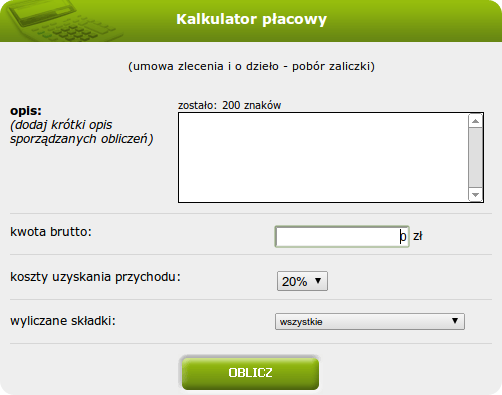
\includegraphics[scale=.6]{img/kalkulator.png}
	\caption{Kalkulator wybagrodzeń z tytułu umów cywilno-prawnych}
	\label{kalkulator}
    \end{center}
\end{figure}

\subsection[SystemUmów.pl][SystemUmów.pl]{SystemUmów.pl}
SystemUmów.pl jest dedykowaną aplikacją internetową frmy KotKla do obsługi umów zleceń oraz o dzieło. Zapewnia ona przede wszystkim:
\begin{itemize}
	\item dodawanie oraz archiwizację umów,
	\item szablony umów(bogata baza dostępnych szablonów oraz możliwość definiowania własnych),
	\item dodawanie pracowników oraz przechowywanie ich danych,
	\item ręczne generowanie rachunków na podstawie szablonów(wbudowanych lub zdefiniowanych własnoręcznie),
	\item export umów i rachunków do formatu pdf,
	\item miesięcznie oraz roczne deklaracje PIT i ZUS,
	\item możliwość definiowania danych (takich jak nazwa, adres, NIP czy REGON) własnej firmy.
\end{itemize}

Jest to aplikacja płatna(150 zł za rok badź 3000 zł za licęcję dożywotnią), ale istnieje też jej darmowa wersja. Charkteryzuje się ona następującymi ograniczeniami:
\begin{itemize}
	\item czas trwania licencji ograniczony do 90 dni,
	\item ilość włąsbych szablonów ograniczona do 3,
	\item liczba umów ograniczona do 50.
\end{itemize}
Program pozwala na łatwe realizowanie podstawych funkcji związanych z obsługą umów cywilno prawnych, łatwo jednak zauważyć kilka podstawowych ograniczeń.
\begin{itemize}
	\item możliwość generacji tylko jednego rachunku do każdej umowy - ogranicza to możliwość ratalnej wypłaty wynagrodzenia.
	\item reczna generecja rachunku na podstawie szablonu pozwala wygenerewać rachunek nie adekwatny do umowy(np. rachunek informujący o 50\% koszcie uzyskania przychodu do nieautorskiej umowy.) wymaga też znajomości składek ZUS pracownika przy każdorazoewj generacji.
	\item brak możliwości podziału przedsiębiorstwa na mniejsze jednostki, czy wyodrębniania poszczególnych zadań.
\end{itemize}

Na rysunku \ref{kotkla-systemumow} przedstawiono przykładowy zrzut ekrany z aplikacji SystemUmów.pl

\begin{figure}[tdh]
    \begin{center}
	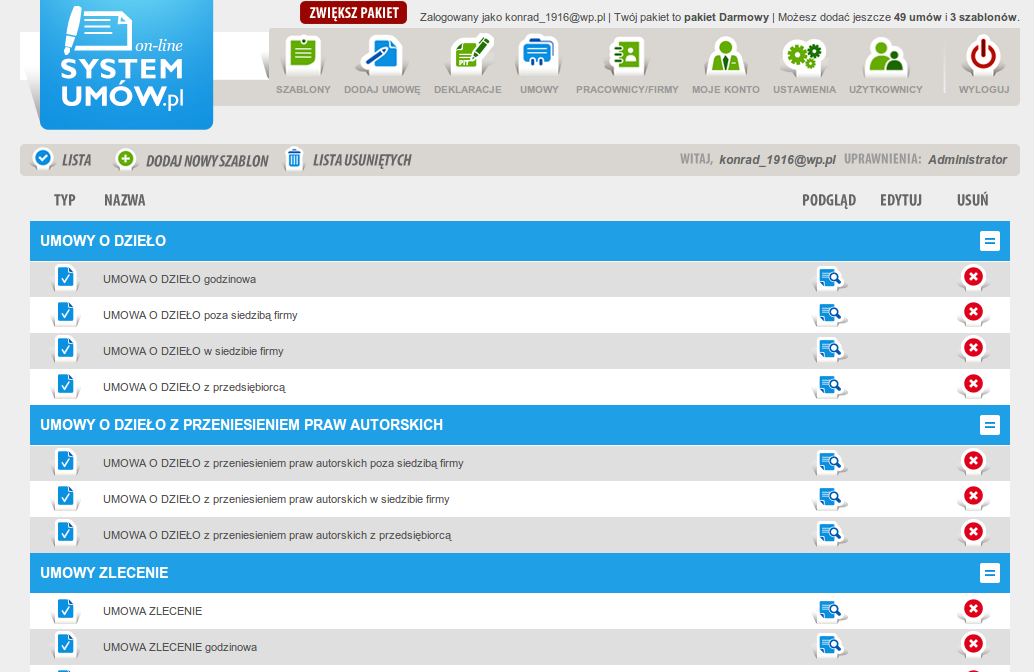
\includegraphics[scale=.4]{img/kotkla-systemumow.png}
	\caption{Lista szablonów umów cywilno-prawnych w aplikacji KotKla-SystemUmów.pl}
	\label{kotkla-systemumow}
    \end{center}
\end{figure}

\subsection[Asystent Rejestr Umów][Asystent Rejestr Umów]{Asystent Rejestr Umów}
Asystent Rejest Umów to program firmy Meteoryt Software. Ma on format aplikacji aplikacji desktopowej korzystającej z bazy danych(lokalnej lub zdalnej). Jest to bardzo zaawansowana aplikacja pozwalająca nie tylko na zarządzanie umowami ale też zaradzanie zadaniami, danynymi kontraktowymi, wspierająca system sprzedarzy czy służąca do fakturowania. Pozwala na obsługę nie tylko umów zleceń czy o dzieło ale też(a raczej przede wszystkim) umów takich jak umowa o pracę czy umowa kupna-sprzedaży. Zepwenia obsługę takich szczegółów jak okres wypowiedzenia czy miejsce prezechowywania oryginału umowy. Pozwala na wysyłanie notyfikacji w formie e-maili bądź smsów. Jest oczywiście aplikacją płatną a jej ceny wachają się w zależności od wersji(najtańszą wersja PRO kosztuje 99zł za rok użytkowania). Na rysunku \ref{asystent-rejestr-umow} przedstawiono przykładowy zrzut ekrany z aplikacji Asystent Rejestr Umów.

\begin{figure}[tdh]
    \begin{center}
	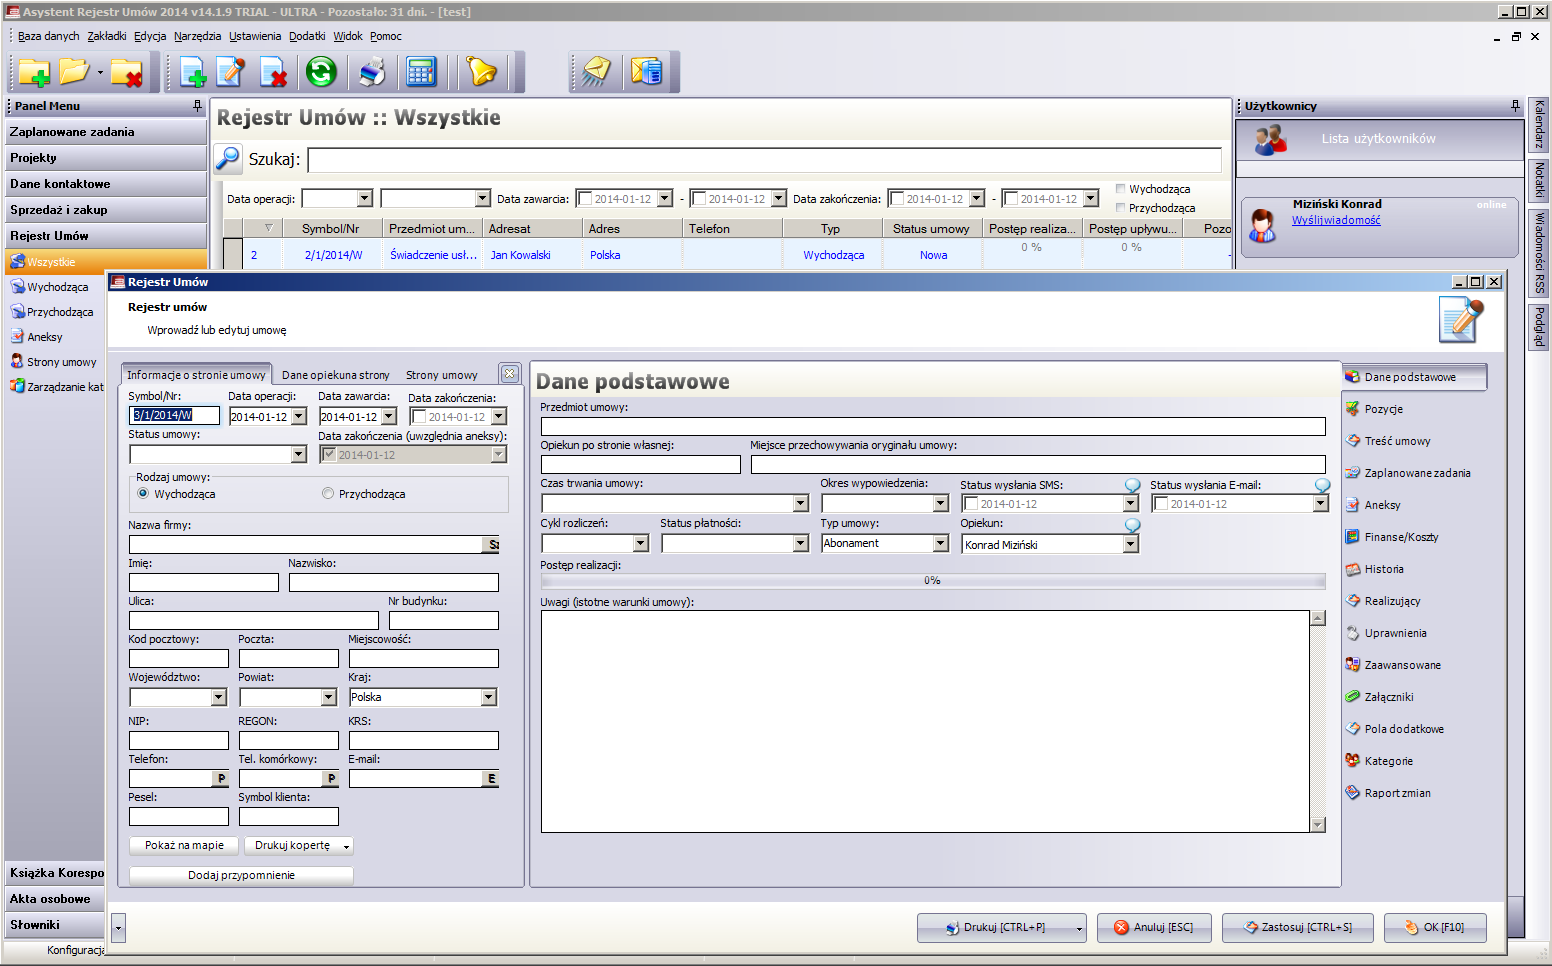
\includegraphics[scale=.6, angle=-90]{img/asystent-rejestr-umow.png}
	\caption{Dodawanie nowej umowy w aplikacji Asystent Rejestr Umów}
	\label{asystent-rejestr-umow}
    \end{center}
\end{figure}

\chapter{Model funkcjonalny}
Poniższy rozdział opisuje proces projektowania aplikacji. Przede wszystkim określa profil odbiorcy sytemu. Prezentuje też wszystkie wymagania jak i założenia poczynione w trakcie ich analizy.

\section[Profil odbiorcy systemu][Profil odbiorcy systemu]{Profil odbiorcy systemu}
Potrzeba stworzenia systemu do obsługi umów cywilno-prawnych powstała na Politechnice Warszawskiej a dokładniej w Ośrodku Kształcenia na Odległość. Początkowa miała ona obsługiwać jedynie umowy zlecenia jednak zdecydowano się ją rozszerzyć również na umowy o dzieło(stąd ogólna nazwa umowy cywilno-prawne). Podczas procesu projektowania starano się jednak aby model był nie tylko dostosowany do specyfiki uczelni ale też jak najbardziej ogólny, tak aby potencjalnym odbiorcą aplikacji mogły być nie tylko uczelnie ale i inne instytucje o podobnej organizacji a nawet małe firmy.

\section[Opis funkcjonalności][Opis funkcjonalności]{Opis funkcjonalności}

\subsection[Pracownicy][Pracownicy]{Pracownicy}
\label{pracownicy}
Aplikacja powinna umożliwiać przechowywanie danych o osobach zatrudnianych na umowach cywilno-prawnych, zwanych dalej potocznie pracownikami(nie są to pracownicy w rozumieniu kodeksu pracy). Podstawowymi operacjami jakie można wykonać na pracowniku jest jego dodanie, modyfikacja oraz usunięcie(ale tylko w przypadku gdy nie ma on podpisanej żadnej umowy). Dodatkowymi funkcjonalnościami są wyszukiwanie pracownika za pomocą imienia i nazwiska oraz możliwość wyświetlenia listy wszystkich pracowników.

Aplikacja będzie gromadzić wszystkie informacje niezbędne jego jednoznacznej identyfikacji, umieszczane na umowach oraz potrzebne w celach podatkowych: nazwisko, imiona(z wyróżnieniem pierwszego imienia), adresy(przy czym należy zwrócić uwagę, że adres wykorzystywany w celach podatkowych może różnić się od adresu korespondencyjnego), datę i miejsce urodzenia, płeć, obywatelstwo(aplikacja powinna udostępniać wybór z listy możliwych państw), numery pesel i NIP, numer dowodu osobistego lub paszportu oraz numer konta. Dodatkowo system powinien przechowywać informację o urzędzie skarbowym(jego nazwę i adres) właściwym dla pracownika. Dane urzędu skarbowego powinny być przechowywane niezależnie od danych pracownika tak aby np. w przypadku zmiany adresu jednego z urzędów nie występowała konieczność ręcznej aktualizacji wszystkich odpowiadających mu pracowników a jedynie pojedyncza modyfikacja danych urzędu skarbowego. Podczas wprowadzania bądź modyfikacji danych pracownika użytkownik powinien mieć możliwość wyboru z listy wcześniej zdefiniowanych urzędów skarbowych lub dodania nowego w przypadku jego braku na liście.

Istotnym elementem danych pracownika jest informacja jakie składki ubezpieczeń będzie musiał odprowadzać od potencjalnie podpisanych umów. Aplikacja powinna przechowywać informacje o jego statusie z punktu widzenia umów cywilno prawnych(opisanym w \ref{przykladyOsob}). Powinna też wspomagać użytkownika w trakcie wyboru statusu - wyświetlać ich szczegółowe opisy oraz powiązane z nimi składki ubezpieczeń. Te informacje powinny być również zawarte w raportach prezentujących dane pracownika. Lista dostępnych statusów jest zdefiniowana w momencie instalacji, nie możliwości jej edycji za pomocą aplikacji.

\subsection[Struktura organizacyjna][Struktura organizacyjna]{Struktura organizacyjna}
Struktura organizacyjna uczelni podobnie jak struktura organizacyjna wielu innych instytucji ma formę drzewa. Dla prawie każdej jednostki organizacyjnej można wskazać jednostkę nadrzędną(Wyjątkiem jest jednostka będąca korzeniem drzewa, z reguły jest to sama organizacja, np konkretna uczelnia). Ponadto jednostki na poszczególnych poziomach drzewa posiadają swoje typy. W przypadku Politechniki Warszawskiej są to np. uczelnia, wydział, instytut i zakład. Nie jest jednak wymogiem aby na jednym poziomie drzewa znajdowały się jednostki tylko jednego typu. Na przykład jednostkami podległymi wydziałowi mogą oprócz instytutów być też dziekanat, czy administracja gmachu. Nie ma też wymogu aby jednostką nadrzędną danej jednostki organizacyjnej był jednostka typu, który jest typem bezpośrednio nadrzędnym do jej typu. Na przykład nie wszystkie zakłady muszą podlegać instytutom, niektóre z nim mogą podlegać bezpośrednio wydziałom. 

Aplikacja powinna udostępniać zestaw typów jednostek oraz definiować który typ jest nadrzędny w stosunku do którego. Dane te powinny być zdefiniowane w momencie instalacji i nie powinno być możliwości ich zmiany z poziomu aplikacji. Program powinien umożliwiać dodawanie nowych jednostek organizacyjnych(nadawanie im nazwy), definiowanie ich typów oraz umieszczanie ich w strukturze organizacji(poprzez nadanie jednostek nadrzędnych). Powinien również umożliwiać ich edycję oraz usuwanie(pod warunkiem, że nie spowoduje to osierocenia innej jednostki organizacyjnej oraz w systemie nie ma zdefiniowanych zadań wykonywanych dla tej jednostki(patrz \ref{zadania})). Aplikacja powinna pilnować struktury drzewa oraz zgodności typów jednostek. Powinna też umożliwić wyszukiwanie jednostki za pomocą jej nazwy, oraz wyświetlania wszystkich jednostek obecnych w systemie.

Atrybutami jednostki oprócz wspominanych wcześniej nazwy, typu i miejsca w strukturze organizacji są jej adres oraz reprezentant, którego zadaniem jest podpisywanie umów w imieniu jednostki. Atrybutami reprezentanta są jego imię i nazwisko jednak ze względu pisemną formę umowy należy przechowywać również formę biernika. Jeden reprezentant może być przypisany do kliku jednostek. Tak jak w przypadku urzędu skarbowego podczas wprowadzania bądź edycji jednostki użytkownik powinien mieć możliwość wyboru reprezentanta z listy już wcześniej wprowadzonych lub dodania nowego.

W trakcie analizy podjęto decyzję, że pracownicy nie będą w żaden sposób połączeni z jedną konkretną jednostką(nawet jeśli są w niej na stałe zatrudnieni).

\subsection[Zadania][Zadania]{Zadania}
\label{zadania}
W ramach jednostek organizacyjnych wykonywane są zadania. To na wykonywanie poszczególnych zadań, bądź ich części zatrudnia się pracowników na umowy cywilno-prawne. Podstawowym atrybutem zadania jest jego nazwa. Zadanie może też posiadać swój opis, budżet, datę rozpoczęcia oraz datę zakończenia. O ile opis pełni charakter jedynie informacyjny, to w przypadku pozostałych atrybutów aplikacja powinna sprawdzać czy umowy podpisywane na wykonanie tego zadanie mieszczą się w zdefiniowanych ramach czasowych(data rozpoczęcia i data zakończenia) oraz czy sumaryczna wartość umów nie przekracza budżetu zdefiniowanego dla danego zadania. Dodatkowo istnieje możliwość oznaczenia zadania jako rozliczone skutkująca tym, że nie będzie można podpisywać już żadnych umów na wykonanie tego zadania. 

Podczas analizy ustalono, że powinna istnieć możliwość podziału zadań na mniejsze grupy w ramach jednostki organizacyjnej. Wprowadzono więc kolejny atrybut zadania jakim jest jego typ(definiowany w ramach jednostki). 

Użytkownik powinien posiadać możliwość dodawania i edycji zarówno zadań jak i ich typów. Usuwanie typów zadań możliwe jest tylko wtedy gdy nie ma żadnego zadania danego typu. Analogicznie usunąć zadanie można tylko wtedy gdy w systemie nie ma żadnych powiązanym z nim umów. Dodatkowo system powinien umożliwiać wyszukiwanie zadań po nazwie oraz ich typie, oraz wyświetlanie wszystkich zadań powiązanych z daną jednostką organizacyjną oraz jednostkami jej podległymi. Analogicznie użytkownik powinien mieć możliwość wyszukiwania typów zadań po ich nazwach oraz możliwość wyświetlania wszystkich typów zadań właściwych dla danej jednostki.

\subsection[Umowy][Umowy]{Umowy}
Najważniejszym obiektem występującym w systemie jest umowa. Podstawowymi atrybutami umowy są jej strony a więc jednostka organizacyjna oraz pracownik. Umowa zawiera też daty zawarcia, rozpoczęcia i zakończenia(przy czym system pilnuje aby data zawarcia była wcześniejsza lub taka sama jak data rozpoczęcia oraz aby data zakończenia późniejsza niż data rozpoczęcia), zawiera również przedmiot umowy(nazwę dzieła lub zlecenia), wynagrodzenie jakie należy się za jego wykonanie oraz informację czy umowa będzie wykonywana w siedzibie zlecającego. 

\subsubsection{Typ umowy}
Użytkownik ma możliwość wyboru typu umowy. Typ umowy definiuje tytuł umowy(umowa zlecenia czy o dzieło) oraz koszt uzyskania przychodu. W projektowanej wersji aplikacji dostępne będą standardowe stawki kosztu uzyskania przychodu wynoszące 20\% i 50\%. Typ umowy posiada również nazwę. Jest ona w ogólnym przypadku różna od tytułu umowy, np. dla typu o nazwie \textit{Umowa o dzieło autorskie} tytułem umowy będzie \textit{Umowa o dzieło}. Na podstawie typu oraz wynagrodzenia z tytułu umowy, a także na podstawie statusu, wieku oraz płci pracownika określane będzie jakie składki będą musiały być odprowadzone od umowy. W przypadku składek dobrowolnych użytkownik pytany jest czy pracownik jest zainteresowany ich odprowadzaniem. Typy umowy są zdefiniowane w systemie w momencie instalacji. Analogicznie do innych elementów tego typu nie ma możliwości ich edycji za pomocą aplikacji.

\subsubsection{Płatność}
Użytkownik ma możliwość wyboru jednego ze zdefiniowanych sposobu płatności. Podstawowym sposobem płatności jest płatność jednorazowa po zakończeniu umowy. System umożliwia też wybór ratalnego sposobu płatności, gdzie okres między kolejnymi ratami może być zdefiniowany w dniach albo miesiącach. Użytkownik ma możliwość samodzielnego definiowana sposobów płatności podając ich nazwę oraz liczbę dni lub miesięcy co jakie powinno być wypłacane wynagrodzenie. Ma też możliwość usuwania zdefiniowanych przez siebie wcześniej a nie używanych sposobów płatności. 

\subsubsection{Numer umowy}
Numery umów będą nadawane automatycznie przez aplikację. Sygnatura umowy powinna być unikalna w skali całego systemu. Przyjęto założenie, że częścią składową numeru umowy będzie data jej zawarcia(w formie numerycznej). Numer umowy będzie umieszczany w jej nagłówku.

\subsubsection{}
Użytkownik ma możliwość dodawania nowych umów, ich edycji oraz usuwania. System umożliwia ponadto wyświetlanie listy wszystkich umów dostępnych dla danego użytkownika oraz pozwala na ich wyszukiwanie na podstawie pracownika, jednostki oraz zadania.

\subsection[Rachunki][Rachunki]{Rachunki}
Jako postawę do wypłaty wynargodzeniea przyjęto rachunki. Rachunki występują zawsze w kontekście danej umowy. Są one ponadto numerowane(nr rachunków są kolejnymi liczbami naturalnymi). Atrybutami rachunku są ponadto kwota oraz data wystawienia.

Rachunki będą generowanie przez aplikację automatycznie na podstawie wybranego sposobu płatności. Użytkownik będzie miał jedynie możliwość ich wyświetlania. Usunięcie rachunków możliwe jest jedynie przez usunięcie powiązanej z nimi umowy, a ich modyfikacja może odbywać się poprzez zmianę parametrów umowy(wynagrodzenia i sposobu płatności).

\subsection[Wydruki][Wydruki]{Wydruki}
Użytkownik będzie miał możliwość wydruku zarówno umów jak i rachunków. Zrealizowane zostanie to poprzez udostępnienie ich w formacie pff. Wydruki umów będą generowane wg wzorców różnych dla każdego typu umowy.

\section[Aktorzy][Aktorzy]{Aktorzy}
W aplikacji zostali wyróżnieni dwaj aktorzy:

\subsubsection{Administrator jednostki}
Powiązany z konkretną jednostką organizacyjną, ma możliwość wykonywania operacji na zadaniach, typach zadań oraz umowach w ramach swojej jednostki oraz wszystkich jednostek jej podlegających. Może mieć możliwość wykonywania operacji na pracownikach.
%TODO co z pracownikami

\subsubsection{Administrator systemu}
Ma możliwość wykonywania operacji na jednostkach organizacyjnych oraz zarządzania administratorami jednostek(ich dodawanie, usuwanie oraz przydzielanie uprawnień). Może definiować nowe sposoby płatności. Ma uprawnienia administratora jednostki dla wszystkich jednostek organizacyjnych obecnych w systemie.

\section[Przypadki użycia][Przypadki użycia]{Przypadki użycia}
Jednym z etapów modelowania aplikacji jest określenie przypadków użycia(ang. \textit{Use Case}). Przypadkami użycia nazywamy funkcjonalności systemu z punktu widzenia użytkownika. Przypadki użycia mogą się w sobie zawierać oraz się rozszerzać. Z punktu widzenia przejrzystości dokumentacji dobrą praktyką jest numerowanie przypadków użycia.

\subsection[Diagram przypadków użycia][Diagram przypadków użycia]{Diagram przypadków użycia}
Diagram przypadków użycia jest graficzną formą ich prezentacji. Zawiera on jedynie aktorów oraz funkcjonalności modelowane systemu. Nie dostarcza informacji o sposobie realizacji tych funkcjonalności. Przykładowy diagram przypadków użycia zamieszczono na rysunku \ref{diagram-uc}.


\begin{figure}[tdh]
    \begin{center}
	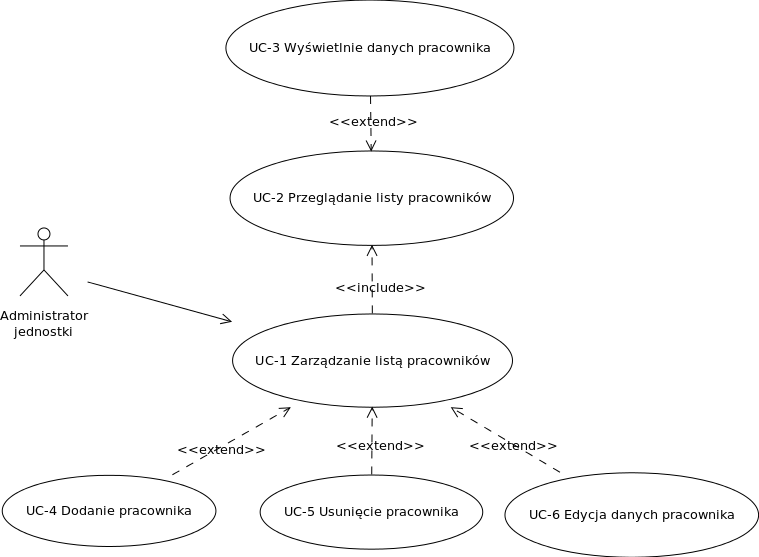
\includegraphics[scale=.6]{img/diagram-uc.png}
	\caption{Diagram przypadków użycia dla zarządzania listą pracowników}
	\label{diagram-uc}
    \end{center}
\end{figure}


\subsection[Scenariusze przypadków użycia][Scenariusze przypadków użycia]{Scenariusze przypadków użycia}
Więcej informacji o poszczególnych funkcjonalnościach system dostarczają scenariusze przypadków użycia. Opisują one w sposób słowny aktorów biorących udział w danych przypadku oraz warunki wstępne oraz końcowe. Opisują też szczegółowo interakcję pomiędzy użytkownikiem a systemem. Wyróżnić można dwie formy takiego opisu: opis w postaci ciągłego tekstu oraz listę kroków. Poniżej przykładowy scenariusz dla przypadku dodawania pracownika:

\paragraph{UC-4 Dodawanie pracownika}
rozszerza UC-1 zarządzanie listą pracowników.\\
\begin{tabular}{ll}
	\textbf{Aktorzy:} & Administrator jednostki \\
	
	\textbf{Warunek początkowy:} & Użytkownik zalogowany w systemie \\
	\textbf{Warunek końcowy:} & Nowy pracownik zapisany w systemie \\
	\multicolumn{2}{l}{\textbf{Scenariusz głowny:}}\\
	\multicolumn{2}{l}{
	\begin{minipage}{\textwidth}\begin{enumerate}
		\item Użytkownik wybiera opcję "Dodaj nowego pracownika".
		\item System wyświetla formularz dadawania użytkownika.
		\item Użytkownik wypełnia formularz.
		\item Użytkownik potwierdza przesłanie formularza przyciskiem "Wprowadź".
		\item System sprawdza poprawność wprowadzonych danych.
		\item System zapisuje dane nowego pracownika
	\end{enumerate}\end{minipage}
	}
\end{tabular}
	
\section[Prototypowanie][Prototypowanie]{Prototypowanie}
Ostatnim etapem fazy analizy jest stworzenie makiet realizowanego systemu. Makiety nie odzwierciedlają faktycznego wyglądu aplikacji, zawierają jednak wszystkie jej elementy w postaci uproszczonych kontrolek. Pozwalają na szersze spojrzenie na całość projektowanego systemu co niekiedy może prowadzić do wychwycenia błędów w jej modelu logicznym. Makiety są wreszcie cenną pomocą dla programistów mających mniejsze doświadczenie w pracy nad częścią kliencką aplikacji. Na rysunku \ref{makieta} przedstawiono przykład makiety formularza do wprowadzania danych pracowników. Została ona wygenerowana za pomocą programu Pencil.

\begin{figure}[tdh]
    \begin{center}
	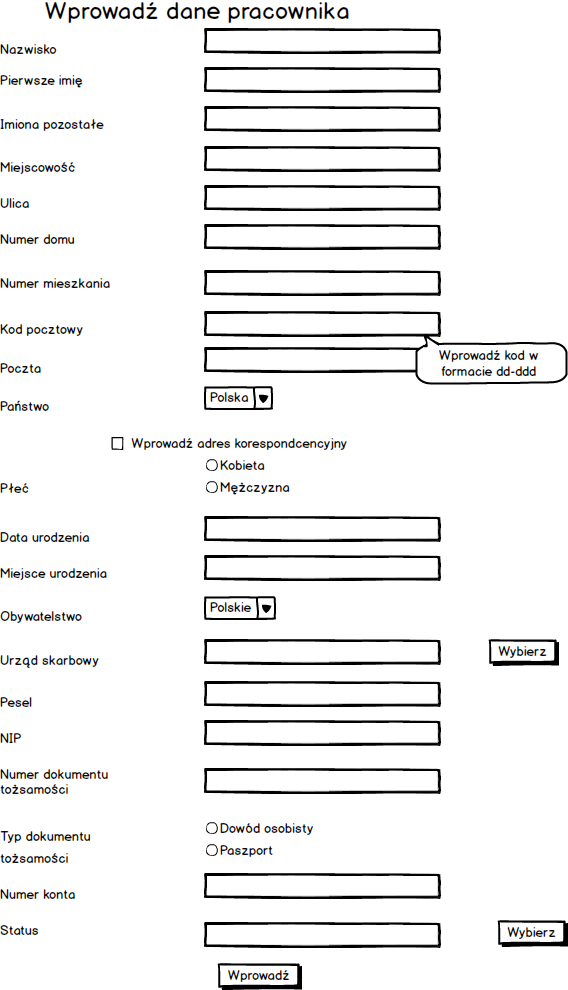
\includegraphics[scale=.8 ]{img/makieta.png}
	\caption{Makieta formularza do wprowadzania danych pracowników}
	\label{makieta}
    \end{center}
\end{figure}


\appendix

% tutaj załączniki

%\chapter*{Bibliografia}
\nocite{*}
\bibliographystyle{plplain}
%\bibliographystylebk{plplain}
%\bibliographystylest{plplain}
%\bibliographystyledoc{plplain}
% \bibliographystyleweb{plplain}
%\bibliographybk{BIB/books}
%\bibliographyst{BIB/books}
%\bibliographydoc{BIB/books}
% \bibliographyweb{BIB/books}

% \bibliography{bib/verificard,bib/jml,bib/daikon}
\bibliography{bib/daikon,bib/statistics,bib/other}

\end{document}

% ex: set tabstop=4 shiftwidth=4 softtabstop=4 noexpandtab fileformat=unix filetype=tex spelllang=pl,en spell:

